\subsection{Retrieval Results}

Table~\ref{tab:retrieval-results} reports the stage-wise Retrieval
evidence. The pool columns are not interchangeable with the submitted
variable-depth measure. Table~\ref{tab:retrieval-cutoff} isolates the
cutoff change from the later deep-tail reranking.

\begin{table*}[tb]
\centering
\caption{Representative Retrieval configurations on the 22-topic
development set. The rows are not a strictly cumulative ablation: the
pool columns and the submitted-depth column refer to different objects,
and only the final two rows are a clean same-pool ordering comparison.
Boldface marks a column maximum, not statistical significance.}
\label{tab:retrieval-results}
\small
\setlength{\tabcolsep}{4.5pt}
\renewcommand{\arraystretch}{1.12}
\begin{tabularx}{\textwidth}{@{}>{\raggedright\arraybackslash}Xrrr@{}}
\toprule
Configuration & Pool $R@1000$ & Pool $R@5000$ & Submitted $R@k_q$ \\
\midrule
Original-narrative BM25 & 0.2635 & --$^{*}$ & -- \\
Query-expanded retrieval with head reranking & 0.2945 & \textbf{0.5155} & -- \\
Facet-expanded retrieval with protected head & 0.3005 & 0.4938 & -- \\
Selected pre-deep-tail retrieval configuration & 0.2937 & 0.4895 & 0.2204 \\
Selected deep-tail retrieval configuration & \textbf{0.3159} & 0.4895 & \textbf{0.2343} \\
\bottomrule
\end{tabularx}
\smallskip

\noindent{\footnotesize $^{*}$The original-narrative baseline was
retrieved only to depth 1,000.}
\end{table*}

\begin{table*}[tb]
\centering
\caption{Variable-depth cutoff comparison on the 22-topic development
set; all values are development diagnostics, not official test-set
results. nDCG uses linear gains after grades below 2 are mapped to zero;
Recall is always Recall@submitted-$k$
in this table. Boldface marks a column maximum, not statistical
significance.}
\label{tab:retrieval-cutoff}
\small
\setlength{\tabcolsep}{6pt}
\renewcommand{\arraystretch}{1.12}
\begin{tabular}{@{}l l r r r r r@{}}
\toprule
Cutoff stage & Submitted depth & nDCG@10 & Recall@submitted-$k$ & MAP & P@10 & MRR \\
\midrule
Historical CE-threshold cutoff & 4--94 & 0.7414 & 0.0563 & 0.0514 & 0.8985 & 0.9848 \\
Relative $\tau=0.20$ & 100--1,000 & 0.7456 & 0.2204 & 0.1389 & 0.9076 & 0.9848 \\
Deep-tail reranking (same depth) & 100--1,000 & 0.7456 & \textbf{0.2343} & \textbf{0.1432} & 0.9076 & 0.9848 \\
\bottomrule
\end{tabular}
\end{table*}


The Retrieval output obtains P@10=0.9076 while submitting fewer than
1,000 documents for 20 of the 22 narratives. Its mean
depth is 601.45, median depth 687.5, and the 18 distinct depths show
that the output is not padded. The fixed-depth comparison is
Recall@1000=0.3159; it is not substituted for Recall@submitted-$k$.

The nDCG@10 increase from 0.7414 to 0.7456 is caused by the cutoff
change rather than by deep-tail reranking. It arises because the
historical CE-threshold cutoff returned only four documents for topic 515, whereas
the relative cutoff exposes ranks 5--10 from the same pre-deep ranking.
That historical cutoff uses sigmoid-transformed cross-encoder logits
stored in the top-100 fusion artifact. It emits four documents when no
artifact entry reaches 0.50 (the archived \texttt{ce\_dead} flag);
otherwise it counts entries with sigmoid score at least 0.50 (the
archived \texttt{ce\_calibrated} field), clips that count to
$[4,5{,}000]$, and takes the corresponding candidate-pool prefix. Its observed
development depths are 4--94. The variable-$k$ scores are computed from
the post-splice, pre-deep-CE candidate-pool scores; Deep CE changes ordering but not the
topic-specific submission depth.

The selected pre-Deep-CE pool has pool Recall@1000=0.2937,
pool Recall@5000=0.4895, and Recall@submitted-$k$=0.2204. Deep-tail
reranking preserves that pool while changing the corresponding values
to 0.3159, 0.4895, and 0.2343, respectively.
In this same-pool comparison, deep-tail reranking improves pool
Recall@1000 without changing pool membership.

\subsection{RAG Results}

The RAG analysis compares stored dense-writing configurations under
different evidence-acquisition and writing settings.
Table~\ref{tab:rag-results} reports the
selected development diagnostics for the three stored RAG configurations
without the internal PS diagnostic; the unreported remainder of FS and
NS is PS.

\begin{table}[tb]
\centering
\caption{Selected RAG development diagnostics for three stored RAG
configurations. These are system variants, not a single-factor
ablation. Boldface marks a column maximum, not statistical significance.}
\label{tab:rag-results}
\small
\setlength{\tabcolsep}{2.5pt}
\renewcommand{\arraystretch}{1.12}
\begin{tabular}{@{}>{\raggedright\arraybackslash}p{2.65cm}rrrr@{}}
\toprule
Configuration & $V_{\mathrm{strict}}$ & $A$ & FS & NS \\
\midrule
12-document-cap baseline & 0.4145 & 0.4862 & 94.8\% & 0.1\% \\
60-document deep-reading & \textbf{0.4698} & \textbf{0.5485} & 95.0\% & 0.1\% \\
Bounded 60-document acquisition (selected) & 0.4656 & 0.5298 & \textbf{97.0\%} & 0.1\% \\
\bottomrule
\end{tabular}
\end{table}

\begin{figure*}[tb]
\centering
\definecolor{resultNavy}{HTML}{24557A}
\definecolor{resultTeal}{HTML}{2A7F78}
\definecolor{resultGray}{HTML}{7B8791}
\begin{minipage}[t]{0.485\textwidth}
\centering
{\small\textbf{(a)} Retrieval ordering at a fixed pool}\par\vspace{1.5mm}
\begin{tikzpicture}[x=1cm,y=1cm,font=\footnotesize]
  \draw[black!35,line width=0.45pt] (2.55,0.50) -- (6.15,0.50);
  \foreach \x/\lab in {2.55/0.20,3.75/0.24,4.95/0.28,6.15/0.32} {
    \draw[black!35,line width=0.45pt] (\x,0.44) -- (\x,0.56);
    \node[anchor=north,text=black!65] at (\x,0.39) {\lab};
  }
  \node[anchor=east,align=right] at (2.36,2.30) {Pool $R@1000$};
  \node[anchor=east,align=right] at (2.36,1.15) {Submitted $R@k_q$};

  \draw[-{Stealth[length=2.2mm]},line width=0.85pt,resultNavy!75]
    (5.361,2.30) -- (6.027,2.30);
  \fill[resultGray] (5.361,2.30) circle (2.1pt);
  \fill[resultNavy] (6.027,2.30) circle (2.7pt);
  \node[anchor=north,text=resultGray] at (5.361,2.17) {0.2937};
  \node[anchor=south,text=resultNavy] at (6.027,2.43) {0.3159};

  \draw[-{Stealth[length=2.2mm]},line width=0.85pt,resultNavy!75]
    (3.162,1.15) -- (3.579,1.15);
  \fill[resultGray] (3.162,1.15) circle (2.1pt);
  \fill[resultNavy] (3.579,1.15) circle (2.7pt);
  \node[anchor=north,text=resultGray] at (3.162,1.02) {0.2204};
  \node[anchor=south,text=resultNavy] at (3.579,1.28) {0.2343};
\end{tikzpicture}
\end{minipage}\hfill
\begin{minipage}[t]{0.485\textwidth}
\centering
{\small\textbf{(b)} RAG coverage--support trade-off}\par\vspace{1.5mm}
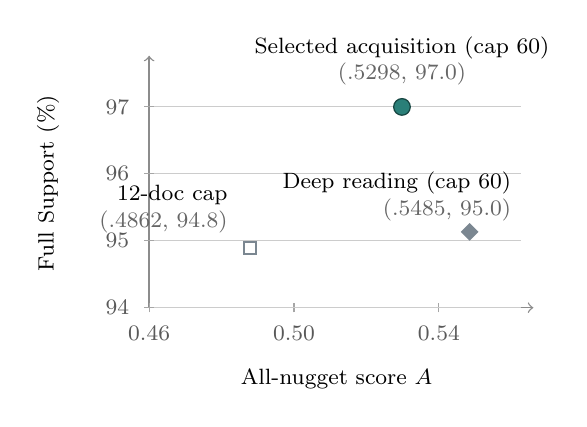
\begin{tikzpicture}[x=1cm,y=1cm,font=\footnotesize]
  \draw[->,black!45,line width=0.5pt] (1.40,0.72) -- (6.28,0.72);
  \draw[->,black!45,line width=0.5pt] (1.40,0.72) -- (1.40,3.92);
  \foreach \x/\lab in {1.40/0.46,3.24/0.50,5.08/0.54} {
    \draw[black!35] (\x,0.66) -- (\x,0.78);
    \node[anchor=north,text=black!65] at (\x,0.61) {\lab};
  }
  \foreach \y/\lab in {0.72/94,1.57/95,2.42/96,3.27/97} {
    \draw[black!20] (1.46,\y) -- (6.12,\y);
    \draw[black!35] (1.34,\y) -- (1.46,\y);
    \node[anchor=east,text=black!65] at (1.27,\y) {\lab};
  }
  \node[anchor=north] at (3.78,0.06) {All-nugget score $A$};
  \node[rotate=90,anchor=south] at (0.38,2.30) {Full Support (\%)};

  \draw[resultGray,line width=0.8pt] (2.605,1.40) rectangle +(4.4pt,4.4pt);
  \node[anchor=south east,align=right] at (2.52,1.55)
    {12-doc cap\\\textcolor{black!60}{(.4862, 94.8)}};

  \fill[resultGray] (5.471,1.57) -- +(3.2pt,3.2pt) -- +(0pt,6.4pt)
    -- +(-3.2pt,3.2pt) -- cycle;
  \node[anchor=south east,align=right] at (6.12,1.70)
    {Deep reading (cap 60)\\\textcolor{black!60}{(.5485, 95.0)}};

  \fill[resultTeal] (4.611,3.27) circle (3.0pt);
  \draw[resultTeal!55!black,line width=0.45pt] (4.611,3.27) circle (3.0pt);
  \node[anchor=south,align=center] at (4.611,3.42)
    {Selected acquisition (cap 60)\\\textcolor{black!60}{(.5298, 97.0)}};
\end{tikzpicture}
\end{minipage}
\caption{Development-set comparison of the selected systems and their
nearest development alternatives. Panel (a) reports the observed change from
pre-deep-tail to deep-tail ordering on the same 5,000-document Retrieval
pool. Panel (b)
plots RAG all-nugget coverage against Full Support; it illustrates the
observed coverage--citation-support trade-off. Exact values and metric definitions appear
in Tables~\ref{tab:retrieval-cutoff} and~\ref{tab:rag-results}.}
\label{fig:development-summary}
\end{figure*}


The 12-document-cap baseline reads five initial documents and up to four
unseen documents per acquisition iteration, with a 12-document cap and
at most three acquisition iterations. Both 60-document configurations
record 12 initial documents, up to ten unseen documents per acquisition
iteration, a 60-document acquisition cap, and at most six acquisition
iterations, plus reranking, passage selection, a supplied checklist, and
verify/revise. The archived deep-reading launcher
sets a 40-document writer limit; the selected development record preserves
neither writer-document nor character limits. Official limits appear in
Appendix~\ref{app:parameters}. The rows are therefore
stored system variants, not a controlled writer-visible-evidence
ablation.

The selected RAG output contains 22 valid and completed topics. Each
topic has 12--30 references, and each answer contains 44--71 answer
objects. The mean answer length is 976.73 words and the maximum is
1,019 words. Table~\ref{tab:output-stats} in
Appendix~\ref{app:structural-stats} reports the corresponding structural
statistics for both systems side by side.

Figure~\ref{fig:development-summary} places the two main comparisons on
their relevant scales. With the 5,000-document Retrieval pool fixed,
deep-tail ordering raises pool Recall@1000 by 0.0222 and
Recall@submitted-$k$ by 0.0139. Figure~\ref{fig:development-summary}
also summarizes the RAG coverage--support trade-off.

\subsection{Answers to the Research Questions}

\textbf{RQ1.}
The selected multi-route pool reaches pool Recall@1000 of 0.2937,
compared with 0.2635 for original-narrative BM25. The original narrative
remains an explicit retrieval route, while the protected splice retains
the top 200 entries of the multi-route, head-reranked pre-facet
ranking before facet-derived candidates are added to the complementary
tail. Deep-tail ordering further raises the same-pool Recall@1000 to 0.3159.

\textbf{RQ2.}
Variable-depth Retrieval produces topic-specific submission depths of
100--1,000 documents, with a mean depth of 601.45 and
Recall@submitted-$k$ of 0.2343; 20 of 22 development topics end below
1,000 documents. The selected RAG configuration bounds evidence
acquisition at 60 documents and at most six evidence-acquisition
iterations and obtains an all-nugget score of 0.5298. The stored RAG
configurations show an observed coverage--support trade-off. We do not
claim a compute-efficiency advantage for variable-depth Retrieval because
runtime cost was not evaluated under a controlled comparison.

\textbf{RQ3.}
The 60-document deep-reading configuration has higher all-nugget
coverage (0.5485 versus 0.5298), whereas the selected bounded
60-document acquisition configuration has higher Full Support (97.0\%
versus 95.0\%). This comparison shows the
coverage--citation-support trade-off observed across the two
configurations, not a Pareto improvement. Because the writer, verifier,
and evidence budgets were not isolated in a single-factor ablation, the
stronger citation support is a property of the selected stored
configuration rather than an identified causal effect of verification.
